\chapter{Implementation}
\label{cha:implementation}
\epigraph{What runs, the code or the comments?}{Brian Kernighan}

\noindent
The code.
With comments being non-executable meta information, Brian Kernighan's question has to be answered with: "the code".
\begin{itemize}
    \item But does it have to be this way?
    \item Is it possible to run comments?
    \item Does it make sense?
    \item Can we blur the lines?
\end{itemize}
As we have seen in Chapters~\ref{cha:introduction} and \ref{cha:related-work}, while the original idea of Hole-Driven Development is closely linked to statically typed functional programming languages, in this chapter we introduce \emph{Holey}\footnote{More information regarding usage and source code can be found at \url{https://holey.dev}.}, our approach on bridging the gap between the type-theoretic formal aspects of Hole-Driven Development and practically applying its ideas to widely used general-purpose programming languages.

\section{Types of Holes}
Until this section, we divided our analysis between todo comments and holes or hole-like alternatives.
If we apply the analogy of a fill-in-the-blanks exercise to programming in general, we can conclude that there is little difference between todo comments, holes, and hole-like alternatives.
They are all blanks that have to be filled in.
But they are not the same; they do have different applications as well as different capabilities.
When we started working on applying hole-driven ideas to \CS at first, we created our own \emph{DSL} (domain-specific language) for writing holes.
After working with this DSL and comparing it with existing solutions and best practices, we quickly realized that while it enabled Hole-Driven Development, it was far off idiomatic \CS-code.
As we identified the idiomatic usage as one of the main properties of holes (compare \ref{hp:idiomatic}), we reverted this approach and examined how existing \CS-features can be re-used as holes.
In this section, we will introduce our classification of the most widely used and applicable types of holes while explaining their usage and use cases. 

\subsection{Todo-Comment}
As seen in Section~\ref{sec:introduction-about-todo-comments}, todo comments are widely used and supported \cite{jetbrains_todo_2023}.
By re-inventing them, legacy code could not be supported, and developers would have to learn a new concept or syntax.
Additional tools for managing todo comments as presented in Section~\ref{sec:tackling-todo-comments} would not be compatible as well.
Furthermore, todo comments are concise to write (\ref{hp:concise}), idiomatic to \CS (\ref{hp:idiomatic}), and allow developers to specify ideas in plain text (\ref{hp:prose-message}).

However, as asked by Brian Kernighan: "What runs, the code or the comments?"
Comments are not intended to be executed; they provide meta-information during development time but not at runtime.
As such, it is essential that they are not missed, which is enabled by emphasizing their existence at compile time (compare Section~\ref{sec:analyzers}, \ref{hp:compile-warnings}).
Although using approaches like source generators (compare Section~\ref{sec:source-generators}), they could actually influence the execution of a program; hence, they could be executed, Holey provides the abstraction of \emph{side effects} (compare Section~\ref{sec:hole-type-side-effect} for this kind of requirement.

Program~\ref{prg:holey-todo-comment} shows the usage of todo comments in \CS.
Nothing about their syntax or usage is specific to Holey.
However, if todo comments exist in a code base using Holey, they get reported as compiler warnings (compare Section~\ref{sec:providing-ide-support}) due to them being unaddressed.

\begin{program}[ht]
\begin{CsCode}
public interface ISidecarConnection
{
	// TODO: get rid of this initialize method; it should be in another interface
	void Initialize();
}
\end{CsCode}
\caption{Usage of a Todo Comment in Holey}
\label{prg:holey-todo-comment}
\end{program}

\subsection{Hole-Comment}
The category of \emph{hole comments} is introduced based upon existing solutions regarding the usage of todo comments like PEP 350 -- Codetags or TagSea (compare Section~\ref{sec:tackling-todo-comments}).
By adding a configurable tag (\ref{hp:taggable}) in brackets after the todo-identifier, todo comments are interpreted as hole comments.
An example of this can be seen in Line~\verb|3| of Program~\ref{prg:holey-hole-comment} where adding \verb|[Refactor]| to the existing todo comment marks it as one that indicates a need for refactoring.
As described by \citeauthor{goldin_stop_2022}, if a todo comment indicates a certain action, it should be specified \cite{goldin_stop_2022}.
This enables developers to categorize todo comments and prioritize them.

At compile time, hole comments are reported using the "information" severity.
This decision was made because they already contain information about how they should be handled.
We hypothesize that this distinction also helps when converting legacy code bases, because by addressing the warnings raised by todo comments one by one, they can be either left as todo comments, enhanced with additional information for handling them later, or directly addressed by getting rid of them.

\begin{program}[ht]
\begin{CsCode}
public interface ISidecarConnection
{
	// TODO [Refactor]: get rid of this initialize method; it should be in another interface
	void Initialize();
}
\end{CsCode}
\caption{Usage of a Hole Comment in Holey}
\label{prg:holey-hole-comment}
\end{program}

\subsection{Missing Implementation}
As Section~\ref{sec:simulating-holes} explains, \texttt{NotImplementedException} is an exception class in \CS's standard library that denotes some implementation is still under development.
Program~\ref{prg:holey-notimplemented} shows the usage of the \texttt{NotImplementedException} where on Line~\verb|6| the default case in a switch-expression is denoted as not implemented.
By not handling all cases, the software\footnote{In this case, the software is Holey itself, which we also develop using the hole-driven approach enabled by Holey.} can already be executed and tested without the need of handling all edge cases.
Not handling edge cases works during development but will probably crash at runtime.
Although IDEs such as Rider show usages of \texttt{NotImplementedException} in the todo window \cite{jetbrains_todo_2023}, they do not surface at compile time.
Similar to todo comments, Holey makes \texttt{NotImplementedException}s visible at compile time by reporting their usages as warnings.
We chose "warning" as the severity for throwing a \texttt{NotImplementedException} because although the program can be run, it will crash once a non-implemented program path is encountered.

\begin{program}[ht]
\begin{CsCode}
holeInformation switch
{
	HoleInformation.EmptyEffect emptyEffect // ...
	HoleInformation.Value value => // ...
	HoleInformation.Effect effect => // ...
	_ => throw new NotImplementedException(\$"{holeInformation.Type} is not handled")
}
\end{CsCode}
\caption{Usage of \texttt{NotImplementedException} in Holey}
\label{prg:holey-notimplemented}
\end{program}

\subsection{Side-Effect}
\label{sec:hole-type-side-effect}
In addition to supporting idiomatic, built-in \CS features, Holey adds the notation of side effect holes.
They correspond most closely to the original definition of holes by resembling executable (\ref{hp:executable}) parts of source code, whose runtime behavior (\ref{hp:runtime-behavior}) can be specified while being further described by a textual message (\ref{hp:prose-message}).
Side-effect holes can be seen as abstract I/O (input and output), which makes them Holey's most powerful abstraction.

Their usage is shown in Program~\ref{prg:holey-side-effects}.
Every value that enters an application and every action that somehow changes the outside world is a side-effect.
After multiple rewrites and simplifications we realized that providing a way to get some value and providing another way to execute an effect is enough to model arbitrary runtime behavior in holes.
As such, a side-effect hole can be introduced using the static method \verb|Hole.Todo(...)|.

By providing a uniform static method to introduce side-effect holes we managed to create a concise notation (\ref{hp:concise}) that also allows holes to be nestable (\ref{hp:nestable}).
As shown in Line~\verb|1| of Program~\ref{prg:holey-side-effects}, Holey has to be imported before it can be used which is limited by the way \CS works, but modern IDEs automatically suggest such usings and \CS 10 enables imports to be defined only once using Global Usings \cite{koch_global_2021}.

\begin{program}[ht]
\begin{CsCode}
using Holey;

var number = Hole.Todo("generate a random number", 42);
var apiKey = Hole.Todo(
	"read the API_KEY from our configuration management service",
	() => Environment.GetEnvironmentVariable("API_KEY")
);
Hole.Todo("validate the incoming data");
await Hole.Todo("save the form data asynchronously", Task.Delay(500));

record User(string Name, int Age);
var user = Hole.Todo("load user data", value => value.Prompt<User>());
\end{CsCode}
\caption{Usage of side-effects in Holey}
\label{prg:holey-side-effects}
\end{program}

As shown in Program~\ref{prg:holey-side-effects}, the first parameter of \verb|Hole.Todo(...)| is a string.
This string acts as the hole's description and lets developers use the informal nature of textual descriptions to describe the intent of the hole.
The second parameter is optional and provides a temporary implementation for the hole.
The type of this second parameter, distinguishes between a hole that provides a value (if \verb|T| is returned) and a hole that executes an effect (if \verb|void| is returned).
This second parameter also distinguishes multiple overloads of the static method \verb|Hole.Todo(...)| whose differences are explained in the rest of this section.

\subsubsection{Values and Effects}
Side-effect holes can either provide a value or execute some effect.
This differentiation is based on whether the hole returns something.
Lines~\verb|3-7| and \verb|12| of Program~\ref{prg:holey-side-effects} show how values can be provided using holes.
If the second parameter is either a constant value or a function returning a value, the hole provides this value, by either simply returning the constant or executing the function and return its result.
Lines~\verb|8| and \verb|9| of Program~\ref{prg:holey-side-effects} depict the usage of effects.
Both statements do not return anything.
The hole in Line~\verb|8| does not take a second parameter, which indicates that something (the task described as the first parameter) has yet to be done.
In comparison to a todo comment, this side-effect hole can be inspected at runtime (compare Section~\ref{sec:reporting}).
The hole in Line~\verb|9| simulates the asynchronous saving of some form data.
Similar to the value holes it simply wraps the task, awaits it, and enhances it with reporting functionality.

One might wonder what is novel about wrapping values and functions and simply returning or calling them.
Wrapping them makes them inspectable at compile-time and runtime, which enables Hole-Driven Development using IDE integrations (compare Section~\ref{sec:providing-ide-support}, runtime reporting (compare Section~\ref{sec:reporting}) and extensibility.

\subsubsection{Asynchrony and Laziness}
As visible in Line~\verb|9| of Program~\ref{prg:holey-side-effects}, holes can be made asynchronous and therefore have to be awaited.
This can simply be accomplished by passing \verb|Task<T>| or \verb|Task| as the second parameter, where the former results in a hole that provides a value, where the latter simulates an effect.
Another aspect of side-effect holes is their laziness.
If the hole's temporary content shall be evaluated lazily, a function can be passed as the secondary parameter which is only evaluated once the hole gets executed.
Laziness and asynchrony can also be combined which enables asynchronous holes that are evaluated lazily.

\subsubsection{Extensibility}
One of the features that makes Holey and its side-effect holes so powerful is its extensibility.
Line~\verb|12| of Program~\ref{prg:holey-side-effects} shows how side-effects can be extended.
Both values and effects can be provided by extension methods.
The method \verb|Prompt<T>()| in Line~\verb|12| shows such an extension by prompting for a user via Holey's Sidecar (compare \ref{sec:sidecar}) application.
These extension can be defined as custom \CS-libraries and allow Holey to be customized for specific use-cases.


\section{Architecture}
\label{sec:holey-architecture}
At its core Holey is a \CS-library which is supported by .NET-analyzers (compare Section~\ref{sec:analyzers}).
To improve learnability and backwards-compatibility, these analyzers support the inspection of todo comments as well as usages of \verb|NotImplementedException|.
In addition to those, the analyzers also report usage information about the holes provided by the library as well as configurable usage of hole comments.
This library and its accompanying analyzers are supported by a Visual Studio extension and an external Sidecar application.
The Visual Studio extension bridges the analyzer results reported by Holey to Visual Studio's task list.
This guarantees that familiar development practices can be continued and shows how extension for additional integrated development environments can be created.
The Sidecar application extends Holey's side-effect holes with additional runtime features.
It is written as a web application which can connect to the Holey library via different communication channels (e.g., Websockets, \verb|postMessage|-function of iFrames) and display information about the usage of holes as well as interact with the application under development via interactive holes.
It also acts as an example of how Holey can be extended and Hole-Driven Development in general-purpose programming languages can lead to interactive programming.

Figure~\ref{fig:holey-architecture} depicts the interaction between these components visually.
\begin{figure}[ht]
    \centering
    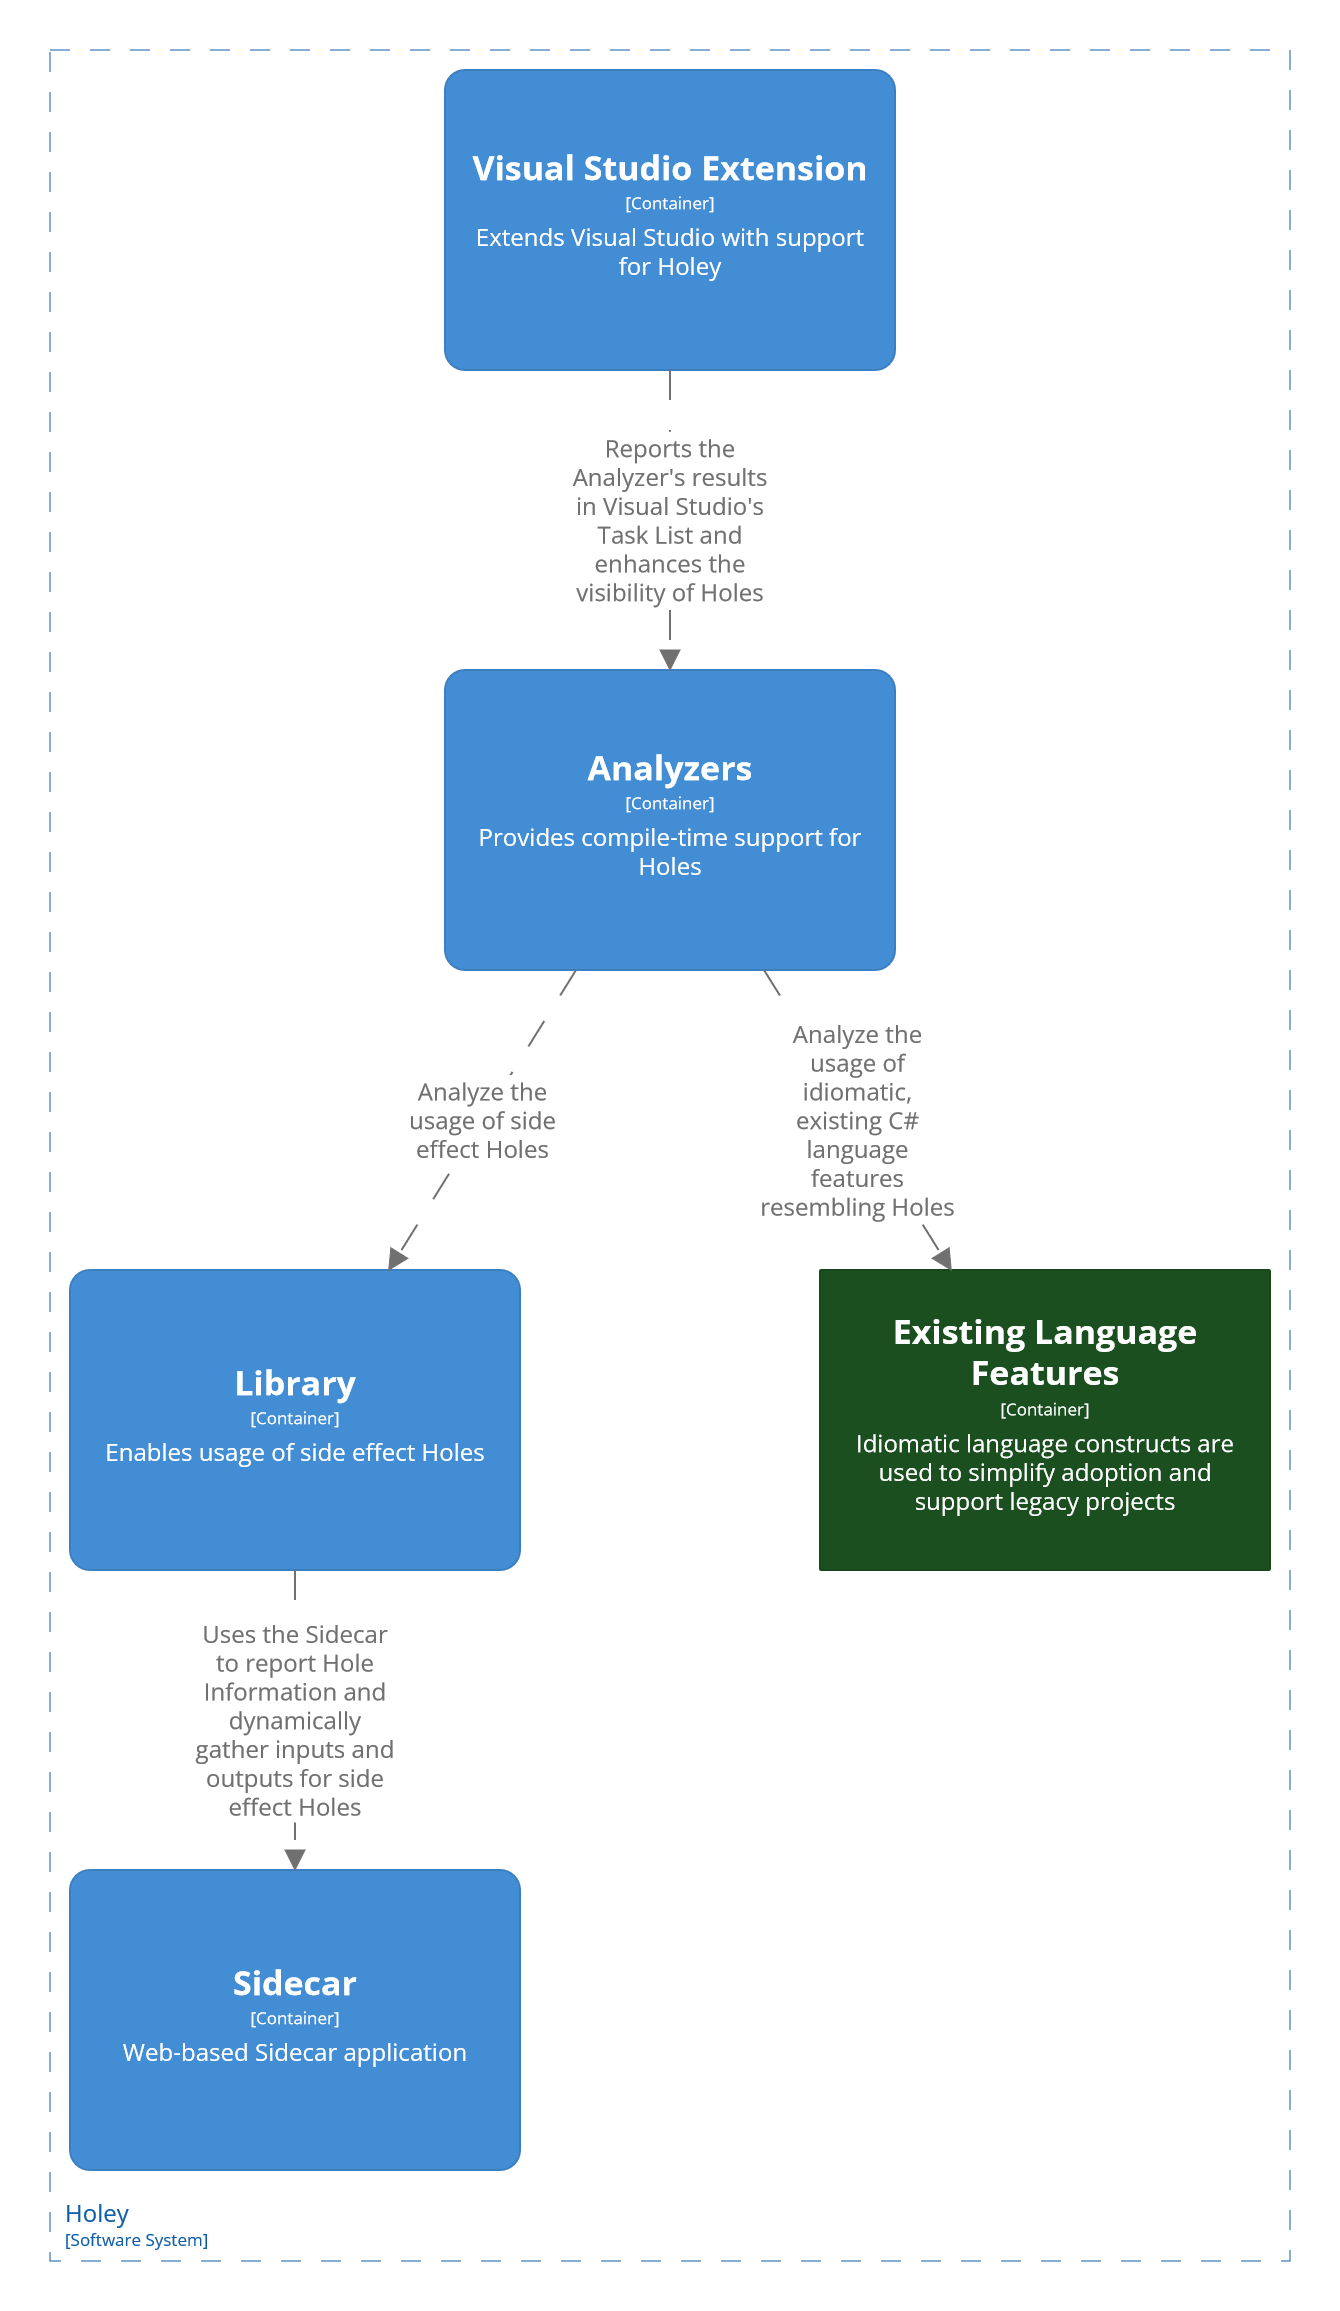
\includegraphics[width=0.97\textwidth]{images/holey-architecture}
    \caption{Overview of the main components of Holey modeled using C4.}
    \label{fig:holey-architecture}
\end{figure}

\subsection{Enabling Configuration}
\label{sec:holey-enabling-configuration}
As explained in Section~\ref{sec:hole-type-side-effect}, Holey provides side-effect holes which affect the runtime behavior of the software under development.

According to \ref{hp:executable} and \ref{hp:runtime-behavior} runtime behavior affecting holes should be configurable, 

Program~\ref{prg:holey-enabling-configuration}

\begin{program}[ht]
\begin{CsCode}
Holes
	.UseLoggerFactory(/*...*/)
	.UseReporting(/*...*/)
	.UseExtensions(/*...*/);
\end{CsCode}
\caption{Configuring the runtime behavior of Holey}
\label{prg:holey-enabling-configuration}
\end{program}

While developing this configuration system we discovered that 

\todo[inline]{Explain the difficulties of bridging the static context and DI}

\subsection{Supporting Logging}
\todo[inline]{Dive into .NET's mess of ILogger, ILogger<T> and ILoggerFactory and their usage in libraries}
\todo[inline]{Explain how this could be solved using StashBox}

\subsection{Enabling Language Independence}
\todo[inline]{Explain the modularity and how the \CS-solution might be transferred to other languages (e.g. Python, Java, TS)}
\todo[inline]{mention what is needed for other languages to adopt holes}
todo comments
exceptions
linters

\section{Providing IDE Support}
\label{sec:providing-ide-support}
\todo[inline]{Give a quick introduction into Roslyn Analyzers}
\todo[inline]{Explain how Roslyn Analyzers offer IDE-independent support}

\begin{figure}[ht]
    \centering
    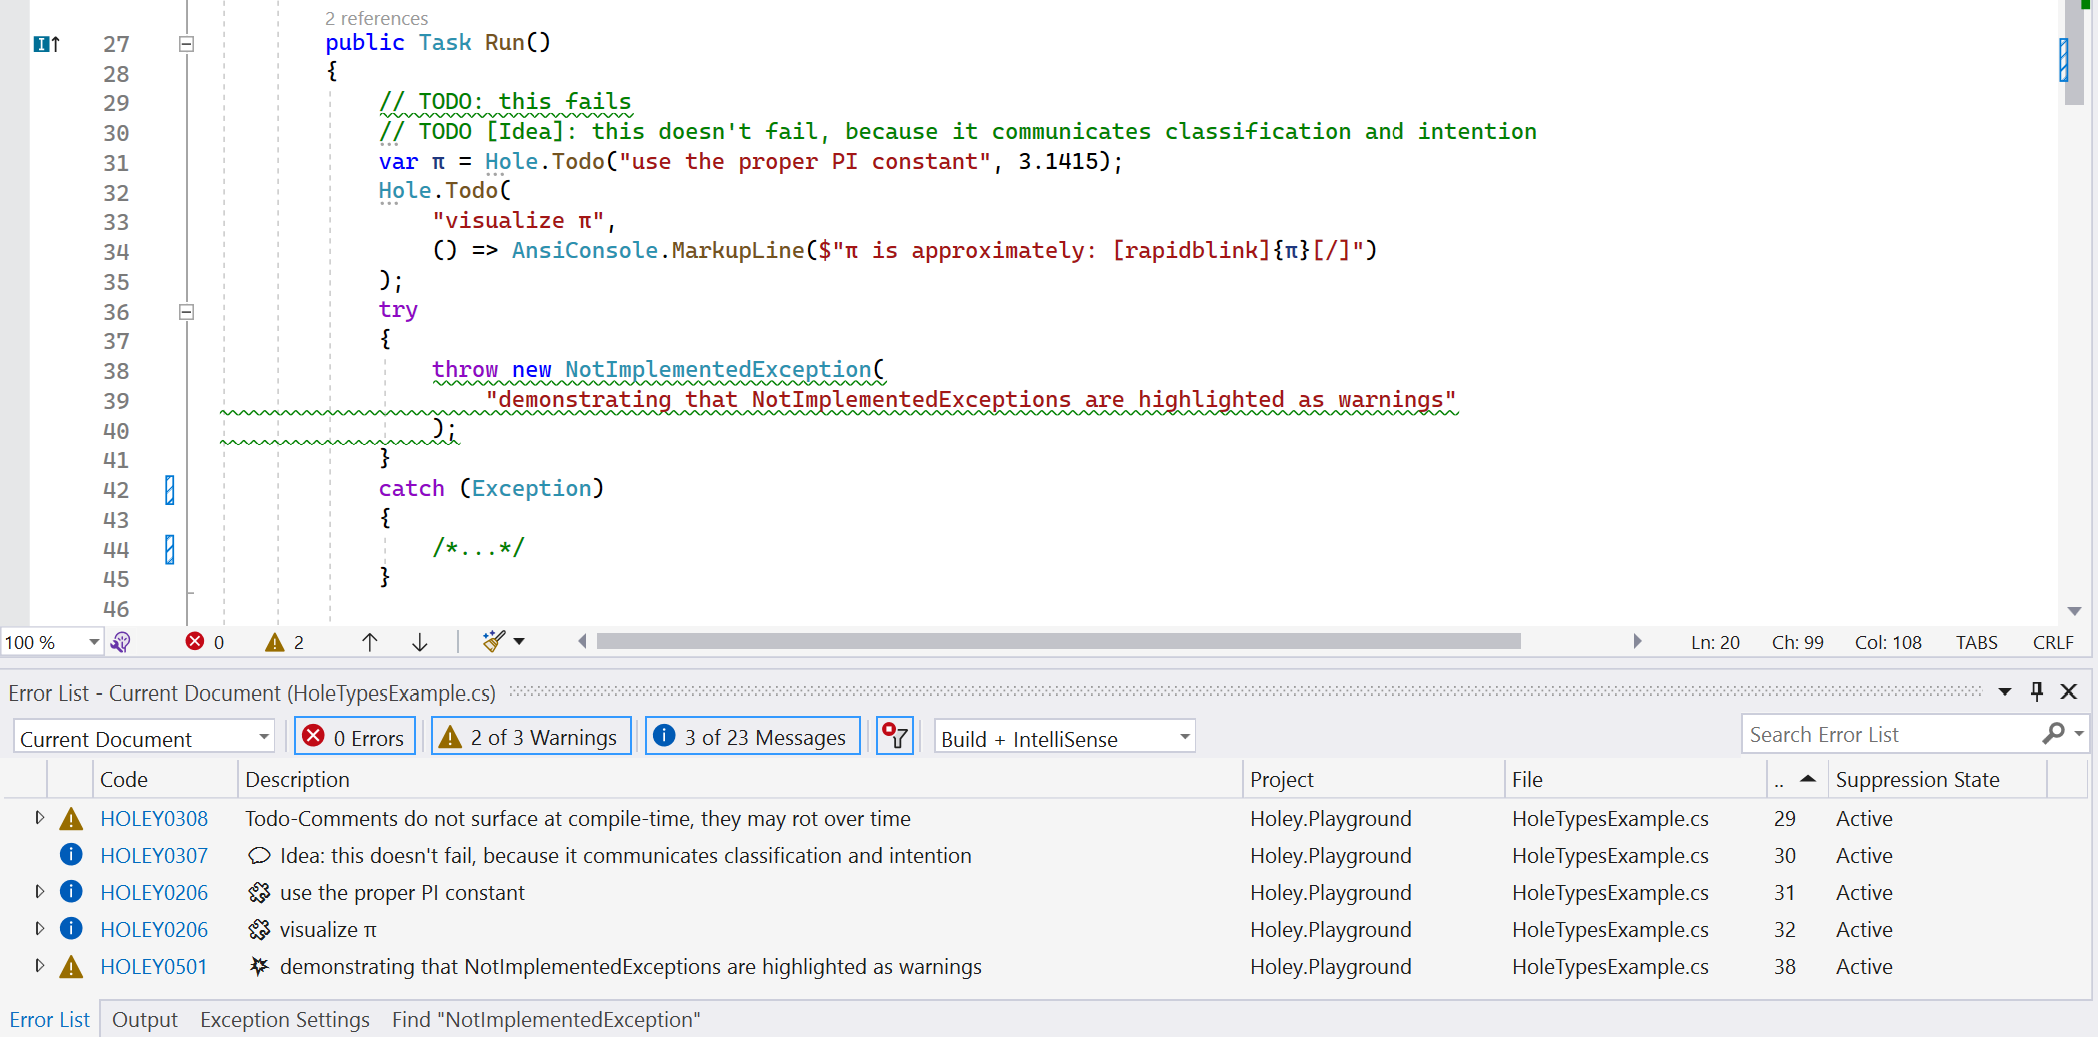
\includegraphics[width=0.97\textwidth]{images/ide-reporting}
    \caption{TODO}
    \label{fig:providing-ide-support}
\end{figure}

\subsection{Analyzers}
\label{sec:analyzers}
\ref{hp:editor-independence}
\ref{hp:compile-warnings}
\todo[inline]{Explain the implemented Analyzers}
\todo[inline]{Explain why it makes sense that debug and release mode are handled separately and how this was accomplished}
\todo[inline]{Connect this to TreatWarningsAsErrors \ref{hp:severity-modes}}
\todo[inline]{Explain the difference to simple linters and define them}

type extraction: \ref{hp:matchable-via-types}

\subsection{Code Fixes}
\todo[inline]{Show the power and usability improvements that Code Fixes in combination with Analyzers provide}
\ref{hp:supported-editor-actions}

\begin{figure}[ht]
    \centering
    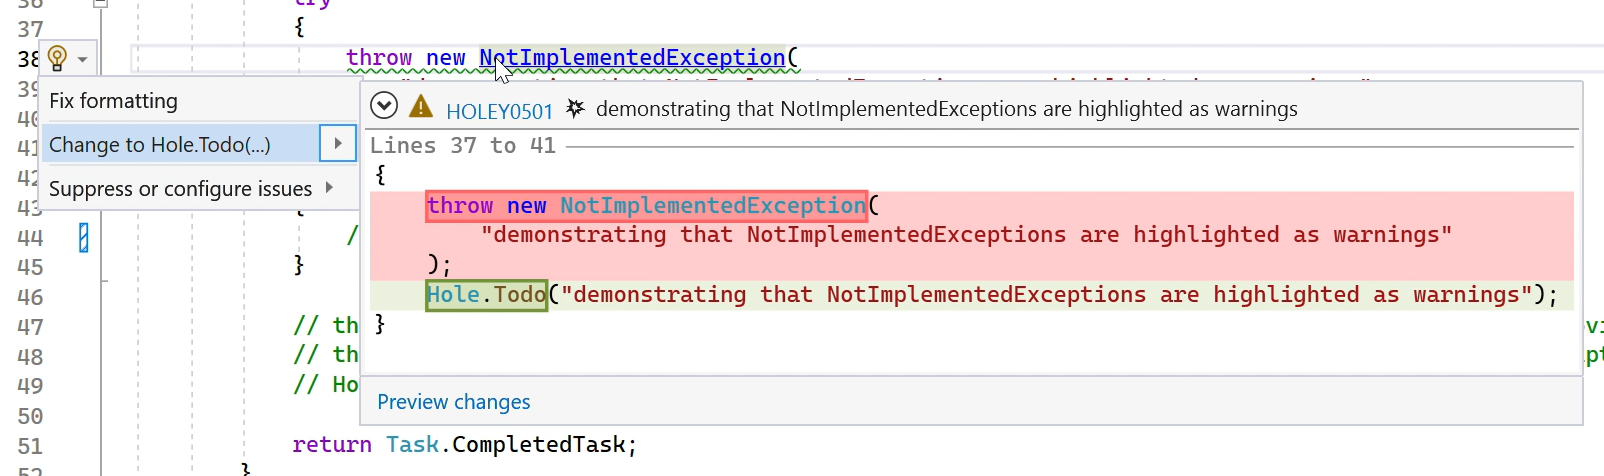
\includegraphics[width=0.9\textwidth]{images/code-fixes}
    \caption{TODO}
    \label{fig:holey-code-fixes}
\end{figure}

\section{Bridging Compile- and Runtime}
\todo[inline]{Explain why it is necessary to bridge between compile- and runtime}

\subsection{Stack Traces}
\todo[inline]{Dig into the concept of Stacktraces and why they might be (but in reality can't) be used to get information about the running code}

\subsection{Compiler Generated Attributes}
\todo[inline]{Explain the usage of .NET's compiler generated attributes}
\todo[inline]{Also mention the downside of having to specify generics when strings are used}

\begin{program}[ht]
\begin{CsCode}
Holes
	.UseLoggerFactory(/*...*/)
	.UseReporting(/*...*/)
	.UseExtensions(/*...*/);
\end{CsCode}
\caption{Configuring the runtime behavior of Holey}
\label{prg:holey-enabling-configuration}
\end{program}

\subsection{Source Generators}
\label{sec:source-generators}
\todo[inline]{Briefly explain \CS's version of source generators vs. T4 templates}
\todo[inline]{Explain how compile-time information can be lifted into runtime}

\begin{program}[ht]
\begin{CsCode}
Holes
	.UseLoggerFactory(/*...*/)
	.UseReporting(/*...*/)
	.UseExtensions(/*...*/);
\end{CsCode}
\caption{Configuring the runtime behavior of Holey}
\label{prg:holey-enabling-configuration}
\end{program}

\section{Extensibility}

Holey can be extended in various ways.


\todo[inline]{Focus on the importance of Extensibility for such an abstract concept/library}

\subsection{Reporting}
\label{sec:reporting}
\todo[inline]{Explain how custom reporters can be utilized}

\subsection{Mocking}
\todo[inline]{Explain the pathway to prototype-mocking as well as why custom packages aren't necessary anymore}
\todo[inline]{Once again mention the concept of abstract I/O and how powerful this is}
\todo[inline]{Transition to the Sidecar Application}

\subsection{Sidecar Application}
\label{sec:sidecar}
\todo[inline]{Briefly explain that the Sidecar Application is no fundamental part of Holey, but it can be created solely on Holey's extensibility options}

\subsubsection{Communication}
\todo[inline]{Explain the abstracted communication channels and that they are not tied to anything else}

\subsubsection{Dynamic Form Generation}
\todo[inline]{Quickly dive into dynamic form generation and show all the code (because it is just one line per application)}
\todo[inline,color=blue!40]{Maybe also mention that the JSON Schema adapter can be switched to a custom one}
\ref{hp:visually-editable}